\section{Message Distribution System (MDS)}

\subsection{Sub topics}

\begin{itemize}
	\item Messaging distribution system - Why \& how?
	\item The PostOffice design - Why and how?
	\item Decoupling achieved.
	\item Design considerations \& implementation.
	\item Patterns per design and in relation to the MDS and PostOffice design:
	\begin{itemize}
		\item GoF Singleton Pattern
		\item GoF Observer Pattern
		\item GoF Mediator Pattern
	\end{itemize}
\end{itemize}

\subsection{Curriculum}

\begin{itemize}
	\item Slides: "A message system".
	\item OLA: "GoF Singleton pattern".
	\item OLA: "GoF Observer pattern".
	\item OLA: "GoF Mediator pattern".
\end{itemize}

\subsection{Exercises}

\begin{itemize}
	\item The Message Distribution System
\end{itemize}

\subsection{Message Distribution system - Why \& how?}

\subsection{The Postoffice Design - Why and how?}

\subsection{Design considerations and implmentation.}

\subsection{Patterns per design and in relation to the MDS and Postoffice design:}

\subsubsection{GoF Singleton Pattern}

\subsubsection{Gof Observer Pattern}

\subsubsection{GoF Mediator Pattern}
Når objekters funktionalitet distribueres ud mellem hinanden, vil der opstå høj kobling, og masser af interkonnektivitet.  I et mediator pattern oprettes et separat mediator-objekt, som står for at kontrollere objekters interaktioner med hinanden. 

\paragraph{Løsning}

\begin{figure}[h]
	\centering
	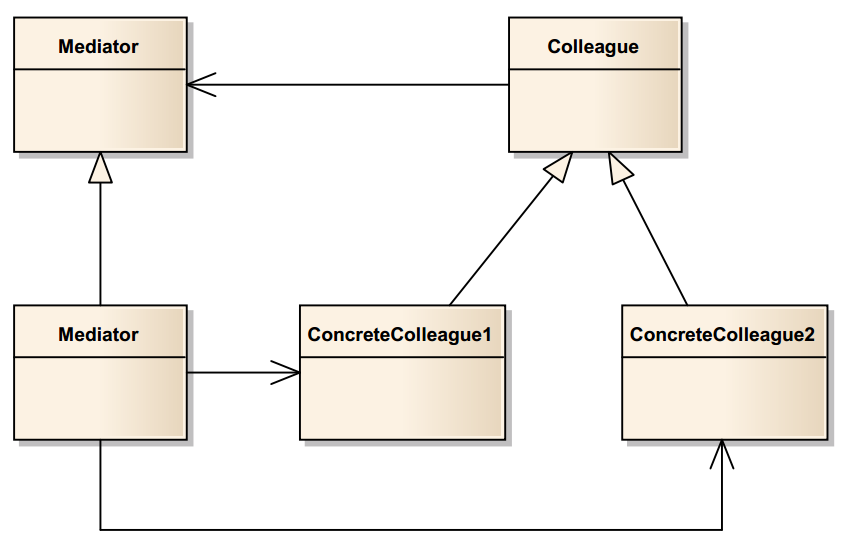
\includegraphics[width=0.8\linewidth]{figs/spm5/concrete}
	\caption{Generelt klassediagram om Mediator pattern.}
	\label{fig:concrete}
\end{figure}

Definition og identifikation af deltagende klassers type:

\begin{itemize}
	\item Mediator.
	\begin{itemize}
		\item 	Definerer et interface til kommunikation med “Colleague objekter”.
	\end{itemize}
	\item Concrete mediator.
	\begin{itemize}
		\item 	Implementerer kommunikationsinterfacet, ved at koordinere Colleague objekter.
	\end{itemize}
	\item Colleague klasser.
	\begin{itemize}
		\item Hver colleague klasse kender sit mediator object.
		\item Når colleaguen vil snakke med en anden klasse, kommunikeres der udelukkende gennem mediatoren.
	\end{itemize}
\end{itemize}

Brugen af et mediator pattern begrænser mængden af afledte klasser i et system, i og med mediatoren centraliserer funktionalitet der ellers ville være spredt ud på mange klasser. Ved at pakke objekters interkonnektivitet ind i et mediator pattern, får man samtidig skabt et ekstra abtraktionsniveau der gør funktionalitet mere overskuelig.

\paragraph{Sammenligning}

Mediator patternet kan sammenlignes med \textbf{publisher-subscriber}. Begge står for at håndtere kommunikationen mellem to eller flere klasser. Hvor publisher-subscriber blot broadcaster til alle subscribers, så har mediatoren i højere grad funktionalitet til at finde ud af, hvilke "colleague" eller "subscribers" der skal udføres noget på. Wiki har et glimrende eksempel på siden om Mediator, som viser, at alt efter hvilken kommando der kaldes, så udfører mediatoren noget forskelligt, og kalder metoderne hos de registrerede objekter med forskellige parametre.

\paragraph{Konsekvenser}
Mediatoren samler en masse funktionalitet på ét sted, hvilket har den fordel at interaktionen mellem objekter bliver nemmere, men mediatoren får derved større ansvar og bliver mere kompleks. Mediatoren kan derfor hurtigt blive en monolit, som er svær at vedligeholde.

\paragraph{Konklusion}
Ud fra journalen kan det konkluderes, at Mediator pattern er godt at bruge, i tilfælde, hvor der opstår mange forbindelser mellem mange forskellige klasser. Ved hjælp af mediatoren centraliseres referencerne til de forskellige objekter ét sted, og samler kald til mediatoren, i stedet for enkelte klasser. Dog skal der passes på at mediatoren ikke bliver til en monolit, hvis for meget funktionalitet bliver pakket ind i den.
